% ============================================================
%  [쉽게 읽는 판] 우주 방사선이 인공지능의 숫자 하나를 바꾸면 무슨 일이 생길까?
%  원 논문: main.tex (같은 그림·같은 수치를 쓴다. 수치 매크로는 tables/numbers.tex 에서 읽음)
%  컴파일: latexmk -xelatex main_easy.tex
%  대상 독자: 중학생. 수식은 꼭 필요한 두 개만 남기고, 용어는 처음 나올 때마다 풀어 쓴다.
% ============================================================
\documentclass[11pt,a4paper]{article}

\usepackage{kotex}
\IfFontExistsTF{Noto Serif CJK KR}
  {\setmainhangulfont{Noto Serif CJK KR}\setsanshangulfont{Noto Sans CJK KR}}
  {\IfFontExistsTF{Noto Serif KR}
     {\setmainhangulfont{Noto Serif KR}[BoldFont={Noto Serif KR},BoldFeatures={FakeBold=1.3}]
      \IfFontExistsTF{NanumGothic}{\setsanshangulfont{NanumGothic}}{\setsanshangulfont{Malgun Gothic}}}
     {\IfFontExistsTF{NanumMyeongjo}
        {\setmainhangulfont{NanumMyeongjo}\setsanshangulfont{NanumGothic}}
        {\setmainhangulfont{Malgun Gothic}\setsanshangulfont{Malgun Gothic}}}}
\usepackage[margin=25mm]{geometry}
\usepackage{amsmath,amssymb}
\usepackage{graphicx}
\usepackage{booktabs}
\usepackage{caption}
\usepackage{float}
\usepackage{xcolor}
\usepackage{tikz}
\usepackage{enumitem}
\usepackage{url}
\usepackage{listings}
\lstset{language=Python,basicstyle=\ttfamily\footnotesize,commentstyle=\color{black!55},keywordstyle=\bfseries,
        frame=single,framerule=0.3pt,rulecolor=\color{black!40},xleftmargin=8pt,xrightmargin=8pt,
        columns=fullflexible,keepspaces=true,showstringspaces=false,breaklines=true,
        numbers=left,numberstyle=\tiny\color{black!50},numbersep=6pt}
\usepackage[hidelinks]{hyperref}
\usepackage[numbers,sort&compress]{natbib}

\graphicspath{{figures/}}
% 자동 생성: paper/make_figures.py — 손으로 고치지 말 것
\newcommand{\NumTrials}{260}
\newcommand{\NumP}{13}
\newcommand{\NumWeights}{101,632}
\newcommand{\NumBits}{3,252,224}
\newcommand{\CleanAcc}{96.66}
\newcommand{\LeoFlipsPerDay}{3.25}
\newcommand{\PhalfNone}{0.055}
\newcommand{\PhalfClip}{5.61}
\newcommand{\PhalfRatio}{102}
\newcommand{\PhalfNoneDays}{17}
\newcommand{\PhalfClipDays}{1754}
\newcommand{\ExpHitFrac}{25.0}
\newcommand{\SignHitFrac}{3.1}
\newcommand{\MaxSeconds}{0.26}
\newcommand{\pThreeEmFiveNoneMed}{96.7}
\newcommand{\pThreeEmFiveNoneSurv}{1.0}
\newcommand{\pThreeEmFiveNoneCrash}{0.0}
\newcommand{\pThreeEmFiveNoneMin}{96.7}
\newcommand{\pThreeEmFiveNoneK}{4}
\newcommand{\pThreeEmFiveClipMed}{96.7}
\newcommand{\pThreeEmFiveClipSurv}{1.0}
\newcommand{\pThreeEmFiveClipCrash}{0.0}
\newcommand{\pThreeEmFiveClipMin}{96.7}
\newcommand{\pThreeEmFiveClipK}{2}
\newcommand{\pOneEmFourNoneMed}{96.6}
\newcommand{\pOneEmFourNoneSurv}{1.0}
\newcommand{\pOneEmFourNoneCrash}{0.0}
\newcommand{\pOneEmFourNoneMin}{95.1}
\newcommand{\pOneEmFourNoneK}{12}
\newcommand{\pOneEmFourClipMed}{96.7}
\newcommand{\pOneEmFourClipSurv}{1.0}
\newcommand{\pOneEmFourClipCrash}{0.0}
\newcommand{\pOneEmFourClipMin}{96.4}
\newcommand{\pOneEmFourClipK}{10}
\newcommand{\pThreeEmFourNoneMed}{93.4}
\newcommand{\pThreeEmFourNoneSurv}{0.6}
\newcommand{\pThreeEmFourNoneCrash}{0.0}
\newcommand{\pThreeEmFourNoneMin}{26.8}
\newcommand{\pThreeEmFourNoneK}{31}
\newcommand{\pThreeEmFourClipMed}{96.6}
\newcommand{\pThreeEmFourClipSurv}{1.0}
\newcommand{\pThreeEmFourClipCrash}{0.0}
\newcommand{\pThreeEmFourClipMin}{96.4}
\newcommand{\pThreeEmFourClipK}{30}
\newcommand{\pOneEmThreeNoneMed}{67.4}
\newcommand{\pOneEmThreeNoneSurv}{0.4}
\newcommand{\pOneEmThreeNoneCrash}{0.0}
\newcommand{\pOneEmThreeNoneMin}{33.2}
\newcommand{\pOneEmThreeNoneK}{104}
\newcommand{\pOneEmThreeClipMed}{96.6}
\newcommand{\pOneEmThreeClipSurv}{1.0}
\newcommand{\pOneEmThreeClipCrash}{0.0}
\newcommand{\pOneEmThreeClipMin}{96.2}
\newcommand{\pOneEmThreeClipK}{97}
\newcommand{\pThreeEmThreeNoneMed}{40.9}
\newcommand{\pThreeEmThreeNoneSurv}{0.0}
\newcommand{\pThreeEmThreeNoneCrash}{0.0}
\newcommand{\pThreeEmThreeNoneMin}{15.5}
\newcommand{\pThreeEmThreeNoneK}{308}
\newcommand{\pThreeEmThreeClipMed}{96.4}
\newcommand{\pThreeEmThreeClipSurv}{1.0}
\newcommand{\pThreeEmThreeClipCrash}{0.0}
\newcommand{\pThreeEmThreeClipMin}{95.2}
\newcommand{\pThreeEmThreeClipK}{299}
\newcommand{\pOneEmTwoNoneMed}{15.4}
\newcommand{\pOneEmTwoNoneSurv}{0.0}
\newcommand{\pOneEmTwoNoneCrash}{0.2}
\newcommand{\pOneEmTwoNoneMin}{10.0}
\newcommand{\pOneEmTwoNoneK}{1019}
\newcommand{\pOneEmTwoClipMed}{95.5}
\newcommand{\pOneEmTwoClipSurv}{0.9}
\newcommand{\pOneEmTwoClipCrash}{0.0}
\newcommand{\pOneEmTwoClipMin}{83.0}
\newcommand{\pOneEmTwoClipK}{1016}
\newcommand{\pFiveEmTwoNoneMed}{10.0}
\newcommand{\pFiveEmTwoNoneSurv}{0.0}
\newcommand{\pFiveEmTwoNoneCrash}{0.5}
\newcommand{\pFiveEmTwoNoneMin}{7.5}
\newcommand{\pFiveEmTwoNoneK}{5080}
\newcommand{\pFiveEmTwoClipMed}{87.2}
\newcommand{\pFiveEmTwoClipSurv}{0.6}
\newcommand{\pFiveEmTwoClipCrash}{0.0}
\newcommand{\pFiveEmTwoClipMin}{77.5}
\newcommand{\pFiveEmTwoClipK}{5076}
\newcommand{\pOneEmOneNoneMed}{10.0}
\newcommand{\pOneEmOneNoneSurv}{0.0}
\newcommand{\pOneEmOneNoneCrash}{0.9}
\newcommand{\pOneEmOneNoneMin}{10.0}
\newcommand{\pOneEmOneNoneK}{10178}
\newcommand{\pOneEmOneClipMed}{71.0}
\newcommand{\pOneEmOneClipSurv}{0.0}
\newcommand{\pOneEmOneClipCrash}{0.0}
\newcommand{\pOneEmOneClipMin}{51.4}
\newcommand{\pOneEmOneClipK}{10137}
% --- E1-M 모델 크기 축 / 수학 모델 / E3 / E5 ---
\newcommand{\NwLinear}{101,632}
\newcommand{\HitsDayLinear}{3.3}
\newcommand{\CleanLinear}{96.7}
\newcommand{\PhalfNoneLinear}{0.0548}
\newcommand{\KhalfNoneLinear}{56}
\newcommand{\DaysNoneLinear}{17일}
\newcommand{\PhalfClipLinear}{5.6}
\newcommand{\DaysClipLinear}{1,754일}
\newcommand{\ClipGainLinear}{102}
\newcommand{\NwCnn}{220,064}
\newcommand{\HitsDayCnn}{7.0}
\newcommand{\CleanCnn}{98.7}
\newcommand{\PhalfNoneCnn}{0.03}
\newcommand{\KhalfNoneCnn}{66}
\newcommand{\DaysNoneCnn}{9일}
\newcommand{\PhalfClipCnn}{3}
\newcommand{\DaysClipCnn}{937일}
\newcommand{\ClipGainCnn}{100}
\newcommand{\NwCifar}{307,040}
\newcommand{\HitsDayCifar}{9.8}
\newcommand{\CleanCifar}{54.6}
\newcommand{\PhalfNoneCifar}{0.0208}
\newcommand{\KhalfNoneCifar}{64}
\newcommand{\DaysNoneCifar}{7일}
\newcommand{\PhalfClipCifar}{0.3}
\newcommand{\DaysClipCifar}{94일}
\newcommand{\ClipGainCifar}{14}
\newcommand{\NwResnet}{11,172,032}
\newcommand{\HitsDayResnet}{357.5}
\newcommand{\CleanResnet}{39.1}
\newcommand{\PhalfNoneResnet}{0.001}
\newcommand{\KhalfNoneResnet}{112}
\newcommand{\DaysNoneResnet}{7.5시간}
\newcommand{\PhalfClipResnet}{0.01}
\newcommand{\DaysClipResnet}{3일}
\newcommand{\ClipGainResnet}{10}
\newcommand{\BimodalNa}{50}
\newcommand{\BimodalNb}{151}
\newcommand{\QLinear}{0.0086}
\newcommand{\AlphaLinear}{0.56}
\newcommand{\KfiftyALinear}{80}
\newcommand{\KfiftyBNoneLinear}{62}
\newcommand{\MaeALinear}{0.04}
\newcommand{\TfiftyPredNoneLinear}{25일}
\newcommand{\KfiftyBLinear}{5,155}
\newcommand{\BetaLinear}{3.2}
\newcommand{\GainLinear}{84}
\newcommand{\TfiftyPredClipLinear}{1,585일}
\newcommand{\QCnn}{0.0115}
\newcommand{\AlphaCnn}{0.78}
\newcommand{\KfiftyACnn}{60}
\newcommand{\KfiftyBNoneCnn}{48}
\newcommand{\MaeACnn}{0.02}
\newcommand{\TfiftyPredNoneCnn}{9일}
\newcommand{\KfiftyBCnn}{5,994}
\newcommand{\BetaCnn}{2.7}
\newcommand{\GainCnn}{126}
\newcommand{\TfiftyPredClipCnn}{851일}
\newcommand{\QCifar}{0.0163}
\newcommand{\AlphaCifar}{1.24}
\newcommand{\KfiftyACifar}{42}
\newcommand{\KfiftyBNoneCifar}{30}
\newcommand{\MaeACifar}{0.06}
\newcommand{\TfiftyPredNoneCifar}{4일}
\newcommand{\KfiftyBCifar}{758}
\newcommand{\BetaCifar}{1.7}
\newcommand{\GainCifar}{26}
\newcommand{\TfiftyPredClipCifar}{77일}
\newcommand{\QResnet}{0.0068}
\newcommand{\AlphaResnet}{0.48}
\newcommand{\KfiftyAResnet}{101}
\newcommand{\KfiftyBNoneResnet}{99}
\newcommand{\MaeAResnet}{0.04}
\newcommand{\TfiftyPredNoneResnet}{6.8시간}
\newcommand{\KfiftyBResnet}{985}
\newcommand{\BetaResnet}{2.1}
\newcommand{\GainResnet}{10}
\newcommand{\TfiftyPredClipResnet}{3일}
\newcommand{\QMin}{0.0068}
\newcommand{\QMax}{0.0163}
\newcommand{\AlphaMin}{0.48}
\newcommand{\AlphaMax}{1.24}
\newcommand{\QCommon}{0.0100}
\newcommand{\LrtD}{6.0}
\newcommand{\LrtDf}{3}
\newcommand{\LrtP}{0.110}
\newcommand{\QMedian}{0.0101}
\newcommand{\TfiftyResnetFifty}{2.0시간}
\newcommand{\TfiftyResnetFiftyMin}{121분}
\newcommand{\TfiftyHundredM}{0.5시간}
\newcommand{\TfiftyHundredMMin}{31분}
\newcommand{\EthreeMAE}{0.06}
\newcommand{\EthreeMaxErr}{0.38}
\newcommand{\EthreeN}{38}
\newcommand{\GainENone}{1.0}
\newcommand{\GainEClip}{83.8}
\newcommand{\GainEParity}{509.7}
\newcommand{\GainETmr}{172.8}
\newcommand{\GainEEnsMed}{1.8}
\newcommand{\GainEEns}{0.2}
\newcommand{\KfiftyTmrPred}{9,327}
\newcommand{\PfiftyTmrPred}{9}
\newcommand{\QEtwoLinear}{0.0081}
\newcommand{\SthirtyEtwoLinear}{0.74}
\newcommand{\SthirtyPredLinear}{0.72}
\newcommand{\SthirtyCILinear}{[0.60, 0.85]}
\newcommand{\QEtwoCnn}{0.0094}
\newcommand{\SthirtyEtwoCnn}{0.70}
\newcommand{\SthirtyPredCnn}{0.63}
\newcommand{\SthirtyCICnn}{[0.51, 0.85]}
\newcommand{\QEtwoCifar}{0.0146}
\newcommand{\SthirtyEtwoCifar}{0.53}
\newcommand{\SthirtyPredCifar}{0.48}
\newcommand{\SthirtyCICifar}{[0.34, 0.72]}
\newcommand{\QEtwoResnet}{0.0052}
\newcommand{\SthirtyEtwoResnet}{0.83}
\newcommand{\SthirtyPredResnet}{0.78}
\newcommand{\SthirtyCIResnet}{[0.65, 0.94]}
\newcommand{\EfourCtrl}{96.38}
\newcommand{\EfourKfiftyNone}{98}
\newcommand{\EfourOneEmThreeNoneMed}{95.2}
\newcommand{\EfourOneEmThreeNoneSurv}{0.6}
\newcommand{\EfourOneEmThreeNoneCrash}{0.5}
\newcommand{\EfourOneEmTwoNoneMed}{10.0}
\newcommand{\EfourOneEmTwoNoneSurv}{0.0}
\newcommand{\EfourOneEmTwoNoneCrash}{1.0}
\newcommand{\EfourOneEmOneNoneMed}{10.0}
\newcommand{\EfourOneEmOneNoneSurv}{0.0}
\newcommand{\EfourOneEmOneNoneCrash}{1.0}
\newcommand{\EfourKfiftyClip}{>10,163}
\newcommand{\EfourOneEmThreeClipMed}{96.4}
\newcommand{\EfourOneEmThreeClipSurv}{1.0}
\newcommand{\EfourOneEmThreeClipCrash}{0.0}
\newcommand{\EfourOneEmTwoClipMed}{96.4}
\newcommand{\EfourOneEmTwoClipSurv}{1.0}
\newcommand{\EfourOneEmTwoClipCrash}{0.0}
\newcommand{\EfourOneEmOneClipMed}{95.3}
\newcommand{\EfourOneEmOneClipSurv}{1.0}
\newcommand{\EfourOneEmOneClipCrash}{0.0}
\newcommand{\EfourCnnCtrl}{98.72}
\newcommand{\EfourCnnOneEmThreeNoneMed}{10.0}
\newcommand{\EfourCnnOneEmThreeNoneSurv}{0.0}
\newcommand{\EfourCnnOneEmThreeClipMed}{98.8}
\newcommand{\EfourCnnOneEmThreeClipSurv}{1.0}
\newcommand{\EfourCnnOneEmTwoNoneMed}{10.0}
\newcommand{\EfourCnnOneEmTwoNoneSurv}{0.0}
\newcommand{\EfourCnnOneEmTwoClipMed}{98.7}
\newcommand{\EfourCnnOneEmTwoClipSurv}{1.0}
                  % 원 논문과 같은 수치 매크로 (자동 생성)

\captionsetup{font={small,sf},labelfont={bf,sf},labelsep=period,format=hang,margin=12pt,skip=6pt}
\setlength{\parskip}{4pt}
\linespread{1.08}

\newcommand{\code}[1]{\texttt{#1}}

% 상자: "쉽게 말하면"(비유·풀이), "직접 계산해 보기"(중학교 수학으로 따라 할 수 있는 계산)
\usepackage{framed}
\newcounter{easy}
\newcounter{calc}
\newenvironment{sidebox}[2]{%
  \par\addvspace{6pt}%
  \def\FrameCommand{{\color{#1}\vrule width 2pt}\hspace{9pt}}%
  \MakeFramed{\advance\hsize-\width\FrameRestore}%
  \small\noindent{\sffamily\bfseries #2.}\ \ignorespaces}%
  {\endMakeFramed\addvspace{6pt}}
\NewDocumentEnvironment{easy}{o}{\refstepcounter{easy}\begin{sidebox}{blue!50}{쉽게 말하면 \theeasy\IfValueT{#1}{ (#1)}}}{\end{sidebox}}
\NewDocumentEnvironment{calc}{o}{\refstepcounter{calc}\begin{sidebox}{orange!70}{직접 계산해 보기 \thecalc\IfValueT{#1}{ (#1)}}}{\end{sidebox}}

\title{\texorpdfstring{\LARGE 우주 방사선이 인공지능의 숫자 하나를 바꾸면\\무슨 일이 생길까?\\[6pt]
\large --- 위성에 실린 인공신경망의 비트플립 실험, 쉽게 읽는 판 ---}{우주 방사선이 인공지능의 숫자 하나를 바꾸면 무슨 일이 생길까? (쉽게 읽는 판)}}
\author{\texorpdfstring{이태린$^{1}$ \quad 최재원$^{2}$ \quad 조교: 이유림$^{3}$ \quad 지도교사: 이성진$^{3}$\\[2pt]
\small $^{1}$민락중학교 \quad $^{2}$선덕중학교 \quad $^{3}$대진대학교}{이태린, 최재원, 이유림, 이성진}}
\date{2026년 11월}

\begin{document}
\renewcommand{\figurename}{그림}
\renewcommand{\tablename}{표}
\renewcommand{\refname}{참고문헌}
\renewcommand{\abstractname}{한 쪽 요약}
\renewcommand{\appendixname}{부록}
\renewcommand{\lstlistingname}{목록}
\maketitle

\begin{center}\small
\fbox{\parbox{0.92\linewidth}{\textbf{이 글에 대하여.} 이 글은 같은 제목의 연구 논문(\code{main.tex})을 중학생이 읽을 수 있도록 다시 쓴 것이다. 실험, 그림, 숫자는 모두 원 논문과 같고, 설명하는 말만 바꾸었다. 어려운 낱말은 처음 나올 때 풀어 쓰고, 맨 뒤 부록에 \textbf{용어 사전}을 두었다. 파란 상자 ``쉽게 말하면''은 비유로 다시 설명한 것이고, 주황 상자 ``직접 계산해 보기''는 중학교 수학으로 따라 할 수 있는 계산이다.}}
\end{center}

% ------------------------------------------------------------
\begin{abstract}
\noindent
인공위성에 실린 인공지능은 우주 방사선 때문에 메모리 속 0과 1이 가끔 저절로 뒤바뀌는 일을 겪는다. 이것을 \textbf{비트플립}(bit flip, 한 자리가 뒤집힘)이라고 한다. 우리는 컴퓨터 안에서 이 일을 그대로 흉내 내는 프로그램을 만들어, 손글씨 숫자를 알아보는 인공신경망의 숫자(가중치) \NumWeights{}개를 조금씩 더 많이 뒤집어 가며 정답률이 어떻게 떨어지는지 쟀다. 알아낸 것은 다음과 같다.
\begin{enumerate}[nosep,leftmargin=*]
  \item 뒤집힌 자리가 많아질수록 정답률은 낮아지지만, 서서히가 아니라 어느 순간 \textbf{갑자기} 무너진다.
  \item 똑같은 개수를 뒤집어도 어떤 때는 멀쩡하고 어떤 때는 망가진다. 중간은 거의 없다. 운명을 가르는 것은 ``\textbf{어느 자리}가 뒤집혔는가''이다.
  \item 32자리 가운데 딱 \textbf{한 자리}(지수 맨 윗자리, bit~30)만 위험하다. 그 자리가 뒤집히면 숫자가 $10^{38}$배 또는 무한대가 된다.
  \item 너무 큰 숫자를 잘라 버리는 가장 단순한 방어 \textbf{클리핑}만으로 버틸 수 있는 방사선 양이 약 \PhalfRatio{}배 늘었다. 궤도 노출 시간으로 바꾸면 약 \PhalfNoneDays{}일에서 약 \PhalfClipDays{}일이 된다.
  \item 크기가 110배 다른 네 모델에서, 절반이 망가지는 \textbf{명중 수}는 \KhalfNoneLinear{}--\KhalfNoneResnet{}개로 거의 같았다. 큰 모델은 자리가 많아 더 자주 맞으므로 \textbf{큰 모델이 먼저 망가진다}. ResNet-18급 모델은 방어 없이 하루를 못 버틴다.
  \item 이 모든 것을 ``한 번 맞아 망가질 확률 $q$'' 하나로 요약한 식 $S=(1-q)^k$가 실험 결과를 잘 맞혔고, 식을 맞추는 데 쓰지 않은 궤도 실험도 평균 오차 \EthreeMAE{}로 예측했다.
  \item 방어 여섯 가지를 비교하니 패리티와 TMR이 가장 강했고, 클리핑이 가성비가 가장 좋았으며, 평균을 내는 앙상블은 오히려 해로웠다.
\end{enumerate}
\medskip
\noindent\textbf{주요어:} 우주 방사선, 비트플립, 부동소수점, 인공신경망, 위성, 클리핑
\end{abstract}

% ------------------------------------------------------------
\section{왜 이 연구를 했나}

\subsection{우주에서는 메모리가 저절로 바뀐다}
컴퓨터 메모리는 0 아니면 1을 저장하는 아주 작은 칸(비트)이 수십억 개 모인 것이다. 지상에서는 지구의 자기장과 공기가 우주에서 날아오는 입자를 대부분 막아 주지만, 우주에서는 그렇지 않다. 아주 빠른 양성자나 무거운 이온이 메모리 칸을 지나가면 그 칸의 전기가 흔들려 0이 1로, 1이 0으로 바뀔 수 있다. 이런 일을 \textbf{단일 사건 오류}(single-event upset, 줄여서 SEU)라고 부른다~\citep{baumann2005}. 메모리가 고장 난 것은 아니고, 저장된 값 하나가 잠깐 바뀐 것이다.

지구 둘레를 도는 낮은 궤도(저궤도, 고도 수백 km)에서는 특히 \textbf{남대서양 이상 지역}(South Atlantic Anomaly, SAA)이라는 곳을 지날 때 이런 일이 몰려서 일어난다. 그 위에서는 지구 자기장이 약해 입자가 더 깊이 내려오기 때문이다.

\begin{easy}[비트플립이란]
시험지를 연필로 다 채웠는데, 비 한 방울이 떨어져 답 하나가 번졌다고 생각해 보자. 시험지가 찢어진 것은 아니다. 그런데 번진 자리가 ``3''의 받침이면 별일 아니지만, ``$\times 10^{3}$''의 3이 번져서 ``$\times 10^{8}$''로 읽히면 답이 십만 배 틀린다. 비트플립도 똑같다. 어느 자리가 바뀌느냐가 전부다.
\end{easy}

\subsection{인공신경망은 숫자 덩어리다}
요즘은 위성이 찍은 사진을 위성 안에서 바로 인공지능으로 판독하려는 시도가 늘고 있다. 그런데 인공지능, 정확히는 \textbf{인공신경망}은 결국 아주 많은 숫자의 덩어리다. 입력(예: 손글씨 사진의 픽셀 값 784개)에 수십만 개의 숫자를 곱하고 더해서 ``이건 7이다''라는 답을 낸다. 이 숫자들을 \textbf{가중치}(weight)라고 한다. 가중치는 학습으로 정해지며, 학습이 끝나면 메모리에 저장되어 있다. 우주 방사선이 바로 이 가중치의 비트를 뒤집으면 어떻게 될까? 그것이 이 연구의 질문이다.

\subsection{알고 싶었던 것}
\begin{enumerate}[label=\textbf{질문 \arabic*.},leftmargin=*]
  \item 뒤집히는 자리가 많아질수록 정답률은 어떤 모양으로 떨어질까? 조금씩? 아니면 어느 선을 넘으면 갑자기?
  \item 가중치가 100배 넘게 많은 큰 모델은 더 튼튼할까, 더 약할까?
  \item 여러 방어 방법은 버틸 수 있는 방사선 양을 몇 배나 늘려 줄까?
  \item 모델 크기, 방사선 양, 방어 방법을 넣으면 ``얼마나 버티는지''를 계산해 주는 간단한 식을 만들 수 있을까?
\end{enumerate}

실험하기 전에 세운 예상(가설)은 이렇다. (가) 많이 뒤집힐수록 정답률은 낮아진다. (나) 서서히가 아니라 어떤 구간에서 급격히 무너진다. (다) 피해는 뒤집힌 \emph{개수}보다 \emph{자리}가 결정하므로, 너무 큰 수만 잘라 내도 많이 좋아질 것이다. (라) ``한 번 맞아 망가질 확률''은 모델 크기와 상관없이 거의 일정할 것이다. (마) 그렇다면 큰 모델은 자리가 많아서 더 자주 맞으므로, 같은 조건에서 \emph{큰 모델이 먼저 망가질} 것이다. (마)는 ``큰 모델은 여분이 많아 더 튼튼하다''는 흔한 생각과 반대라서 특히 확인하고 싶었다.

% ------------------------------------------------------------
\section{꼭 알아야 할 배경 지식}

\subsection{컴퓨터는 소수를 어떻게 저장할까}
과학 시간에 아주 큰 수나 작은 수를 $6.02\times10^{23}$처럼 쓰는 법을 배운다. 앞의 $6.02$가 ``얼마''이고, $10^{23}$이 ``자릿수''이다. 컴퓨터도 소수를 이렇게 저장한다. 다만 10진법이 아니라 2진법이고, 32칸(비트)을 쓴다. 이 방식을 \textbf{float32}(32비트 부동소수점)라고 한다~\citep{ieee754}. 그림~\ref{fig:float32}처럼 32칸은 세 부분으로 나뉜다.
\begin{itemize}[leftmargin=*,nosep]
  \item \textbf{부호} 1칸(bit~31): 0이면 양수, 1이면 음수.
  \item \textbf{지수} 8칸(bit~30--23): ``$2$의 몇 제곱''인지. $10^{23}$의 23에 해당한다.
  \item \textbf{가수} 23칸(bit~22--0): ``얼마''에 해당하는 부분. $6.02$에 해당한다.
\end{itemize}
값은 $w=(-1)^{S}\times2^{E-127}\times(1+M/2^{23})$인데, 식 자체보다 중요한 것은 다음 한 가지다. \textbf{어느 칸이 뒤집히느냐에 따라 피해 크기가 하늘과 땅 차이다.}

\begin{figure}[H]
  \centering
  \begin{tikzpicture}[x=0.36cm,y=0.8cm,font=\scriptsize]
    \fill[blue!20]   (0,0) rectangle (1,1);
    \fill[red!20]    (1,0) rectangle (9,1);
    \fill[gray!15]   (9,0) rectangle (32,1);
    \draw (0,0) rectangle (32,1);
    \foreach \i in {1,...,31} \draw[gray!50] (\i,0) -- (\i,1);
    \node at (0.5,0.5) {S};
    \node at (5,0.5) {지수 $E$ (8칸)};
    \node at (20.5,0.5) {가수 $M$ (23칸)};
    \node[above] at (0.5,1) {31};
    \node[above] at (1.5,1) {30};
    \node[above] at (8.5,1) {23};
    \node[above] at (9.5,1) {22};
    \node[above] at (31.5,1) {0};
    \node[below] at (5,0) {bit 30이 뒤집히면: $\times 2^{128}$ 또는 무한대};
    \node[below] at (20.5,0) {가수 칸이 뒤집히면: 값이 2배 이내로만 바뀜};
    \draw[gray] (0.5,0) -- (0.5,-0.9);
    \node[anchor=north west] at (0.5,-0.9) {부호 칸이 뒤집히면: $+$가 $-$로};
  \end{tikzpicture}
  \caption{float32의 32칸. 지수는 32칸 중 8칸뿐이지만 피해의 거의 전부를 만든다.}
  \label{fig:float32}
\end{figure}

\begin{calc}[숫자 $1.0$의 칸을 하나씩 뒤집어 보면]
$1.0$은 부호 0, 지수 $01111111$, 가수 전부 0으로 저장된다. 여기서 칸 하나씩만 뒤집어 보자.
\begin{itemize}[nosep,leftmargin=1.6em]
  \item 가수 맨 아랫칸(bit~0)을 뒤집으면 $1.0000001$. 천만분의 1만 달라졌다. 아무 일도 없다.
  \item 가수 맨 윗칸(bit~22)을 뒤집으면 $1.5$. 가수 칸 중 가장 큰 변화인데도 2배가 안 된다.
  \item 부호 칸(bit~31)을 뒤집으면 $-1.0$. 크기는 그대로, 부호만 바뀐다.
  \item 지수 맨 윗칸(bit~30)을 뒤집으면 지수가 $11111111$이 되어 \textbf{$+\infty$(무한대)}가 된다. $1.0$ 대신 $0.99$였다면 약 $3.4\times10^{38}$, 즉 1 뒤에 0이 38개 붙은 수가 된다.
\end{itemize}
32칸 중 31칸은 뒤집혀도 값이 2배 이내로 바뀌거나 부호만 바뀐다. 딱 bit~30 한 칸만 $10^{38}$배 또는 무한대를 만든다. 이 사실 하나가 이 연구의 거의 모든 결과를 설명한다.
\end{calc}

\begin{easy}[무한대와 ``숫자 아님'']
컴퓨터는 너무 커서 표현할 수 없는 수를 $\infty$(무한대)라는 특별한 값으로 적어 둔다. 그리고 $\infty-\infty$나 $0\times\infty$처럼 답을 정할 수 없는 계산의 결과는 NaN(Not a Number, ``숫자 아님'')으로 적는다. NaN은 전염성이 있다. NaN이 하나라도 섞인 계산의 결과는 다시 NaN이다. 그래서 가중치 하나가 $\infty$가 되면, 몇 단계 뒤에는 인공신경망의 출력 열 개가 전부 NaN이 되어 아무 답도 낼 수 없게 된다. 이 글에서는 이 상태를 \textbf{붕괴}라고 부른다.
\end{easy}

\subsection{작은 오차는 자라지 않는다, 큰 오차는 처음부터 크다}
``나비효과''라는 말처럼, 작은 오차가 단계를 거치며 눈덩이처럼 불어나지 않을까? 인공신경망에서는 그렇지 않다. 신경망은 ``곱하고 더하기''를 층층이 쌓은 것인데, 오차도 신호와 \emph{같은} 곱셈과 덧셈을 지나간다. 학습이 잘 된 신경망은 신호가 층을 지나며 폭발하거나 사라지지 않도록 만들어져 있으므로, 오차도 대체로 처음 크기 그대로 전달된다. 실제로 우리 실험에서 가수 칸을 뒤집은 작은 오차는 2층짜리 모델부터 18층짜리 ResNet까지 어느 깊이에서도 정답률을 바꾸지 못했다.

그러면 피해는 어떻게 생기는가? 오차가 \emph{자라서}가 아니라 처음부터 \emph{거대해서} 생긴다. bit~30이 뒤집혀 생긴 $10^{38}$ 크기의 값은 다음 층에서 수만 개의 숫자를 더할 때 혼자서 합 전체를 차지해 버린다. 한 층만 지나도 피해는 끝난 것이다.

\begin{easy}[평균은 큰 수 하나에 끌려간다]
반 친구 다섯 명의 용돈이 1만, 1만, 1만, 1만, 1만 원이면 평균은 1만 원이다. 그런데 한 명이 실수로 ``1조 원''이라고 적으면 평균은 2천억 원이 된다. 나머지 넷이 뭐라고 적었든 상관없다. 신경망의 덧셈도 마찬가지다. $10^{38}$ 하나가 들어오면 나머지 수만 개의 가중치가 아무리 많아도 묻혀 버린다. ``큰 모델은 가중치가 많아서 튼튼하다''는 생각이 틀린 이유가 여기 있다.
\end{easy}

\subsection{네 가지 방어 방법}
\begin{itemize}[leftmargin=*]
  \item \textbf{클리핑}(clipping, 자르기): 가중치를 쓰기 전에 NaN은 0으로, 무한대나 $3$보다 큰 값은 $3$으로, $-3$보다 작은 값은 $-3$으로 잘라 낸다. 비트가 뒤집히는 것을 막지는 못하지만, 괴물 같은 값이 다음 층으로 퍼지는 것을 끊는다. 비용이 거의 없다.
  \item \textbf{패리티}(parity, 홀짝 검사): 32칸에 1칸을 더 붙여 ``1의 개수가 짝수가 되도록'' 맞춰 둔다. 나중에 1의 개수가 홀수이면 어딘가 한 칸이 뒤집힌 것이다. 어느 칸인지는 모르므로 그 가중치를 0으로 만들어 버린다. 메모리가 $1/32$, 약 3\,\% 더 든다.
  \item \textbf{TMR}(삼중 모듈 중복): 같은 가중치를 세 벌 저장해 두고, 쓸 때 세 값의 \textbf{중앙값}(크기 순으로 가운데 값)을 쓴다. 한 벌이 무한대가 되어도 가운데 값은 멀쩡하다. 메모리가 3배 든다.
  \item \textbf{앙상블}(ensemble): 모델 전체를 다섯 벌 두고 각각 답을 낸 뒤 합친다. 합치는 방법이 \textbf{평균}이면 한 벌만 망가져도 전체가 끌려가고(위의 용돈 예), \textbf{중앙값}이면 셋 이상이 망가져야 끌려간다. 메모리가 5배, 계산도 5배 든다.
\end{itemize}

\begin{easy}[TMR과 앙상블은 무엇이 다른가]
둘 다 ``여러 벌을 두고 합친다''는 점은 같다. 차이는 \emph{언제} 합치느냐다. TMR은 가중치 하나하나마다 세 벌을 비교해서 계산을 \emph{시작하기 전에} 고친다. 앙상블은 다섯 모델이 각자 계산을 \emph{끝낸 뒤} 답을 합친다. 끝난 뒤에는 이미 망가진 모델의 답이 $10^{38}$이나 NaN이라서, 평균으로 합치면 그 하나가 나머지 넷을 삼킨다. 그래서 같은 중앙값이라도 TMR이 훨씬 세다.
\end{easy}

% ------------------------------------------------------------
\section{어떻게 실험했나}

\subsection{비트플립 시뮬레이터}
우주에 갈 수는 없으므로, 컴퓨터 안에서 메모리의 비트가 뒤집히는 일을 그대로 흉내 내는 프로그램(\code{seu\_suite})을 파이썬으로 만들었다. 핵심은 목록~\ref{lst:flip}의 세 줄이다. (1) 신경망의 가중치를 메모리 그대로 가져오고, (2) 그 메모리를 ``소수''가 아니라 ``32칸짜리 0/1 묶음''으로 다시 읽은 뒤, (3) 원하는 칸 하나를 뒤집는다(XOR). 복사본을 만들지 않고 메모리 제자리에서 바꾸므로 신경망이 쓰는 가중치가 진짜로 바뀐다. 프로그램을 켤 때마다 ``$1.0$의 bit~31을 뒤집으면 $-1.0$, bit~30을 뒤집으면 $+\infty$''가 되는지 스스로 점검한다.

\begin{lstlisting}[float=htb,caption={비트플립의 핵심 세 줄(\code{src/radiation.py}의 \code{xor\_one\_bit}을 줄인 것).},label={lst:flip}]
w = weight.detach().numpy()           # (1) 가중치를 메모리 그대로 가져온다 (복사 없음)
u = w.view(np.uint32).ravel()         # (2) 같은 메모리를 32칸짜리 0/1 묶음으로 다시 읽는다
u[i] ^= np.uint32(1) << np.uint32(b)  # (3) i번째 가중치의 b번째 칸을 뒤집는다
\end{lstlisting}

\begin{easy}[가우시안 잡음과 무엇이 다른가]
다른 연구에서는 ``모든 가중치에 작은 무작위 수를 더하는'' 방법(가우시안 잡음)으로 손상을 흉내 내기도 한다. 그것은 비가 온 시험지 전체가 고르게 살짝 번진 상황이다. 진짜 방사선은 그렇지 않다. 딱 한 칸이 바뀌고, 그 결과는 어느 칸이냐에 따라 천만분의 1배에서 $10^{38}$배까지 달라진다. 그래서 우리는 진짜로 칸을 뒤집었다.
\end{easy}

\subsection{방사선의 양: $p$와 궤도에서의 날수}
실험에서 방사선의 양을 조절하는 손잡이는 $p$다. $p$는 \textbf{가중치 하나가 명중될 확률}이다. 명중된 가중치는 32칸 중 무작위로 한 칸이 뒤집힌다. 예를 들어 $p=0.1\,\%$이면 가중치 1,000개 중 약 1개가 맞고, 가중치가 \NumWeights{}개인 모델에서는 약 100개가 맞는다. 이렇게 맞은 가중치의 수를 \textbf{명중 수} $k$라고 부른다. 평균적으로 $k=p\times(\text{가중치 수})$이다.

그런데 $p$는 실험용 손잡이일 뿐, 우주에서 실제로 얼마나 자주 일어나는지는 따로 알아야 한다. 저궤도 위성에 실린 보통 메모리를 실제로 재 보니, 비트 하나가 하루에 뒤집힐 확률은 약 백만분의 1($r=10^{-6}$/bit/day)이었다~\citep{bentoutou2008}. 적어 보이지만 메모리 1\,GB(약 86억 비트)이면 하루에 약 8,600칸이 뒤집히는 양이다. 지상에서는 한 달에 몇 번 수준이니 만 배 이상 많다.

이 값을 쓰면 $p$를 ``궤도에서 며칠 지낸 것과 같은가''로 바꿀 수 있다. 하루 명중 수는 $r\times(\text{비트 수})=r\times32\times(\text{가중치 수})$이므로, 기대 명중 수가 같아지는 날수는
\begin{equation}
  T_{\mathrm{eq}}=\frac{p\times(\text{가중치 수})}{r\times32\times(\text{가중치 수})}=\frac{p}{32\,r}
  \label{eq:teq}
\end{equation}
이다. 가중치 수가 약분되어 사라지므로, 이 환산은 모델 크기와 관계없이 같다.

\begin{calc}[$p$를 날수로 바꾸기]
$r=10^{-6}$이면 $32r=3.2\times10^{-5}=0.0032\,\%$이다. 그러므로 $p=0.0032\,\%$가 궤도 하루, $p=0.01\,\%$가 약 3일, $p=0.1\,\%$가 약 31일이다. 뒤에 나오는 ``절반이 망가지는 $p$''인 \PhalfNone\,\%는 약 \PhalfNoneDays{}일에 해당한다. 그림의 위쪽 눈금이 이 환산이다. 다만 $r$은 고도·메모리 종류·태양 활동에 따라 몇 배씩 달라지므로, 날수는 ``$r=10^{-6}$일 때''의 값이다.
\end{calc}

\subsection{실험에 쓴 네 모델}
주된 모델은 손글씨 숫자 데이터 MNIST~\citep{lecun1998}(학습용 6만 장, 시험용 1만 장)를 배운 2층짜리 신경망 \code{mnist\_linear}이다. 깨끗할 때 정답률은 \CleanAcc{}\,\%이고, 뒤집을 수 있는 가중치는 \NumWeights{}개, 비트로는 \NumBits{}개이다. 실험 한 번에 1초가 안 걸려서 여러 조건을 많이 반복할 수 있다.

``큰 모델은 어떤가''를 보기 위해 세 모델을 더 썼다(표~\ref{tab:model}). 합성곱 모델 \code{mnist\_cnn}, 컬러 사진 10종류(CIFAR-10)를 배운 6층 모델 \code{cifar\_deep}, 그리고 1,100만 개가 넘는 가중치를 가진 \code{resnet18\_t10}이다. 마지막 모델은 이미 ImageNet이라는 큰 데이터로 학습되어 배포되는 ResNet-18~\citep{he2016}의 앞부분을 그대로 쓰고 마지막 층만 새로 학습한 것이다. 가장 작은 모델과 가장 큰 모델의 가중치 수는 110배 차이 난다. 뒤의 두 모델은 컴퓨터 시간이 모자라 깨끗할 때 정답률이 낮지만(각 \CleanCifar{}\,\%, \CleanResnet{}\,\%), 우리는 ``깨끗할 때와 비교해서 얼마나 떨어졌나''를 재므로 크기 효과를 보기에는 충분하다.

\begin{table}[H]
  \centering\scriptsize
  \caption{실험에 쓴 네 모델. $N_w$는 뒤집을 수 있는 가중치 수, $N_{\mathrm{bits}}=32N_w$는 비트 수. ``명중/일''은 궤도에서 하루에 맞는 가중치 수($r=10^{-6}$/bit/day). $p_{50}$, $k_{50}$은 절반이 망가지는 $p$와 명중 수, LEO 일수는 식~\eqref{eq:teq}로 바꾼 날수.}
  \label{tab:model}
  \begin{tabular}{lrrrr|rrr|rr}
\toprule
모델 & $N_w$ & $N_{\mathrm{bits}}$ & 무손상 & 명중/일 & \multicolumn{3}{c|}{방어 없음, 생존률 50\%} & \multicolumn{2}{c}{클리핑, 생존률 50\%} \\
 & & & 정확도 & ($r$=$10^{-6}$) & $p_{50}$ (\%) & $k_{50}$ & LEO 일수 & $p_{50}$ (\%) & LEO 일수 \\
\midrule
\code{mnist\_linear} & 101,632 & 3,252,224 & 96.7 & 3.3 & 0.0548 & 56 & 17일 & 5.6 & 1,754일 \\
\code{mnist\_cnn} & 220,064 & 7,042,048 & 98.7 & 7.0 & 0.03 & 66 & 9일 & 3 & 937일 \\
\code{cifar\_deep} & 307,040 & 9,825,280 & 54.6 & 9.8 & 0.0208 & 64 & 7일 & 0.3 & 94일 \\
\code{resnet18\_t10} & 11,172,032 & 357,505,024 & 39.1 & 357.5 & 0.001 & 112 & 7.5시간 & 0.01 & 3일 \\
\bottomrule
\end{tabular}

\end{table}

\subsection{무엇을 쟀나}
한 번 실험할 때마다 네 가지를 기록했다.
\begin{itemize}[leftmargin=*,nosep]
  \item \textbf{정답률}: 손상된 모델이 시험 문제를 몇 \% 맞혔나.
  \item \textbf{붕괴}: 가중치나 출력에 NaN이나 무한대가 하나라도 생겼나. 붕괴하면 정답률은 찍는 수준(10\,\%)으로 적는다.
  \item \textbf{생존}: 붕괴하지 않고, 정답률이 깨끗할 때의 90\,\% 이상이면 ``살아남았다''고 본다. 같은 조건을 10번 반복했을 때 살아남은 비율이 \textbf{생존률}이다.
  \item \textbf{명중 수} $k$와, 그중 지수 칸·부호 칸이 맞은 수.
\end{itemize}
결과를 요약할 때는 평균 대신 \textbf{중앙값}을 썼다. 이유는 \ref{sec:bimodal}절에서 나온다.

\subsection{실험 목록}
\begin{table}[H]
  \centering\small
  \begin{tabular}{llp{8.6cm}}
    \toprule
    이름 & 질문 & 무엇을 했나 \\
    \midrule
    E1 & $p$가 커지면? & \code{mnist\_linear}에 $p$를 $0.001\,\%$부터 $10\,\%$까지 13단계로 바꾸며, 방어 없음과 클리핑 각 10번씩(총 \NumTrials{}번). \\
    E1-M & 큰 모델은? & 같은 실험을 나머지 세 모델에 반복. \\
    E2 & 어느 칸이 위험한가? & 정확히 한 칸만 한 번 뒤집기. 부호·지수 8칸·가수 4칸을 각각 30--50번. \\
    E3 & 진짜 궤도처럼 몰려서 맞으면? & 하루 명중의 90\,\%를 SAA 통과 3번(각 12분)에 몰아넣은 궤도 모드로 1--90일. 식을 맞추는 데 쓰지 않고 검증에만 썼다. \\
    E5 & 어떤 방어가 좋은가? & 방어 6종(없음, 클리핑, 패리티, TMR, 앙상블 중앙값, 앙상블 평균)을 $p$ 8단계에서 비교. 한계를 보려고 $p=50\,\%$까지도 올려 봤다. \\
    \bottomrule
  \end{tabular}
\end{table}
모든 실험은 난수의 씨앗(시드)을 기록해 두어 누구나 같은 결과를 다시 얻을 수 있다.

% ------------------------------------------------------------
\section{무엇을 알아냈나}

\subsection{많이 맞을수록 틀리는데, 서서히가 아니라 갑자기}
그림~\ref{fig:dose}가 E1의 결과다. 방어가 없을 때, $p=0.01\,\%$(명중 약 12개)까지는 정답률이 \pOneEmFourNoneMed{}\,\%로 깨끗할 때와 같다. $p=0.03\,\%$(명중 약 31개)에서 생존률이 \pThreeEmFourNoneSurv{}로 떨어지기 시작하고, $p=0.1\,\%$에서 중앙값 \pOneEmThreeNoneMed{}\,\%, $p=0.3\,\%$에서 \pThreeEmThreeNoneMed{}\,\%, $p\ge1\,\%$에서는 찍는 수준인 \pOneEmTwoNoneMed{}\,\%가 된다. 가로축이 10배씩 커지는 눈금이라는 점에 주의하자. 정답률은 $p$가 약 10배 커지는 좁은 구간($0.03\,\%\sim0.5\,\%$)에서 거의 다 떨어진다. 예상 (가)와 (나)가 맞았다.

\begin{figure}[!htb]
  \centering
  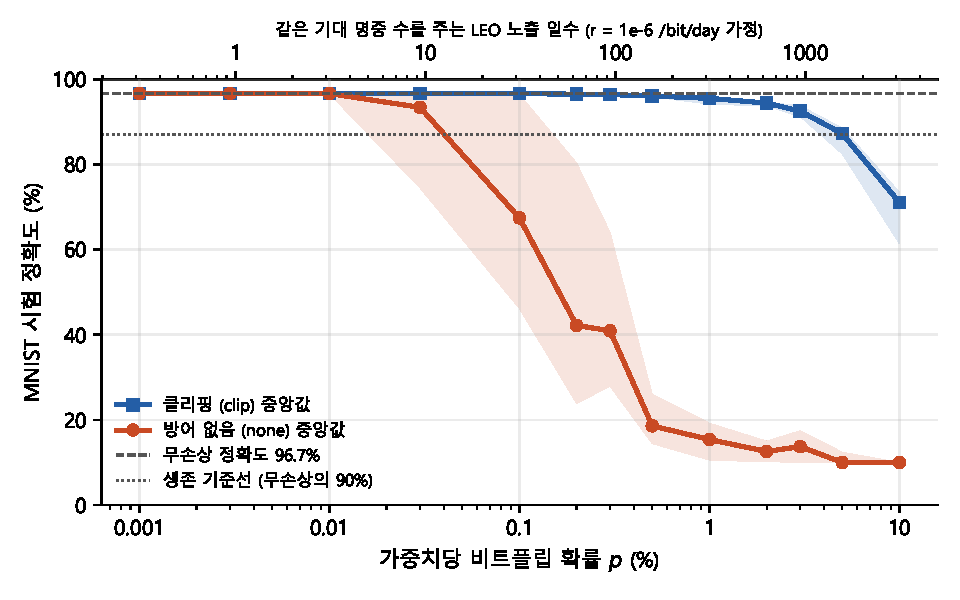
\includegraphics[width=0.95\linewidth]{fig_e1_dose_response}
  \caption{E1: $p$에 따른 정답률. 선은 10번 실험의 중앙값, 색 띠는 가운데 절반이 들어가는 범위. 위쪽 눈금은 식~\eqref{eq:teq}로 바꾼 궤도 날수.}
  \label{fig:dose}
\end{figure}

\subsection{같은 양을 맞아도 운명이 갈린다}
\label{sec:bimodal}
그림~\ref{fig:trials}는 실험 하나하나를 점으로 찍은 것이다. 방어 없음의 $p=0.03\,\%\sim0.3\,\%$ 구간을 보면, 같은 $p$인데도 어떤 점은 96\,\% 근처에 멀쩡하게 있고 어떤 점은 30--70\,\%로 뚝 떨어져 있다. 그 사이는 비어 있다. 예컨대 $p=0.1\,\%$의 10번 중 4번은 96\,\% 이상, 6번은 33--78\,\%였다. 이 구간에서 명중 수는 매번 거의 같다(약 100개). 그러니 차이는 ``몇 개 맞았나''가 아니라 ``\emph{어느 가중치의 어느 칸}이 맞았나''에서 온다.

\begin{figure}[!htb]
  \centering
  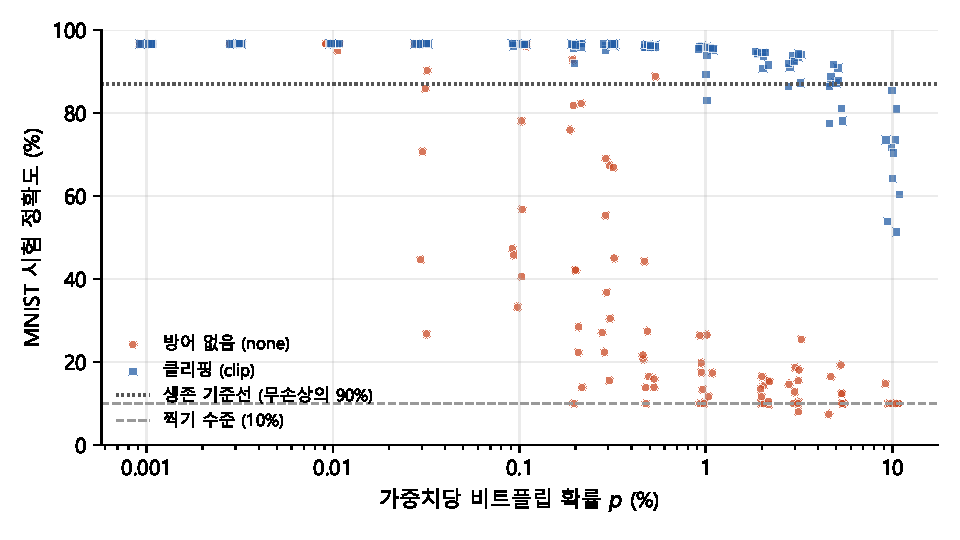
\includegraphics[width=0.95\linewidth]{fig_e1_trials}
  \caption{E1의 모든 실험(점 하나 = 실험 1번). 방어 없음은 중간 구간에서 두 무리로 갈라진다.}
  \label{fig:trials}
\end{figure}

그림~\ref{fig:bimodal}은 이 구간의 결과를 막대그래프(히스토그램)로 모은 것이다. 이 그림만은 $p$마다 100번씩 실험했다. 봉우리가 둘이다. 하나는 깨끗할 때 근처, 하나는 10--80\,\%에 넓게 퍼져 있고, 그 사이 85--93\,\%는 거의 비어 있다. 이런 모양을 \textbf{이봉 분포}(bimodal distribution, 봉우리가 둘인 분포)라고 한다. 네 모델을 합쳐 그려도 같은 모양이고, 같은 양을 맞은 클리핑 실험은 전부 깨끗한 봉우리에 모여 있다.

\begin{figure}[!htb]
  \centering
  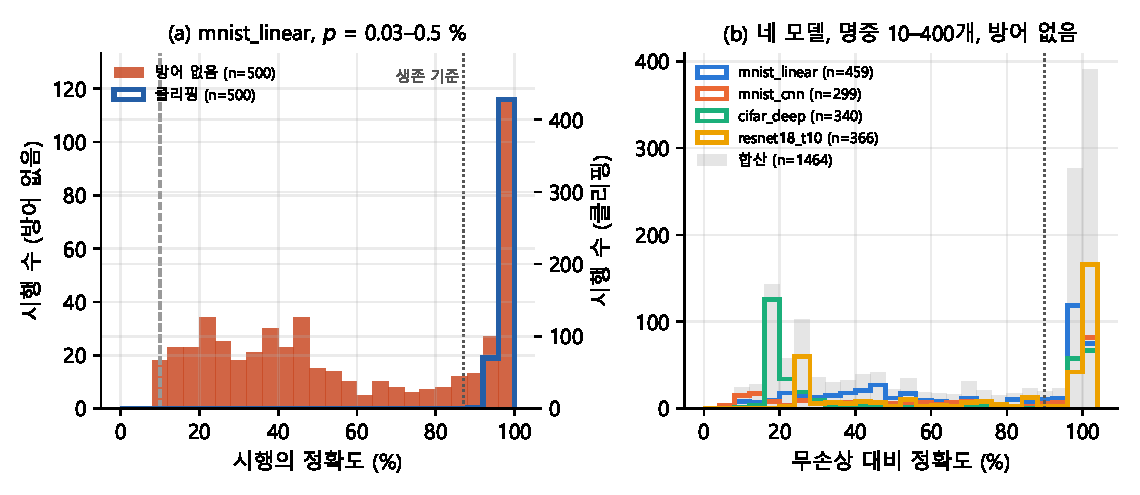
\includegraphics[width=0.95\linewidth]{fig_bimodal}
  \caption{이봉 분포($p$마다 100번 실험). (a) \code{mnist\_linear}의 $p=0.03$--$0.5\,\%$ 구간 \BimodalNa{}번: 방어 없음(채움, 왼쪽 축)과 클리핑(선, 오른쪽 축). (b) 네 모델의 명중 10--400개 구간 \BimodalNb{}번을 깨끗할 때 대비 정답률로 합친 것.}
  \label{fig:bimodal}
\end{figure}

\begin{calc}[왜 봉우리가 둘인가]
명중 하나가 32칸 중 bit~30에 떨어질 확률은 $1/32$, 떨어지지 않을 확률은 $31/32$이다. $k$번 맞는 동안 한 번도 bit~30에 떨어지지 않을 확률은 $(31/32)^k$이다. 계산기로 두드려 보면 $k=31$일 때 약 $0.37$, $k=104$일 때 약 $0.04$이다. 즉 명중 31개면 10번 중 약 4번은 위험한 칸을 피하고, 104개면 거의 못 피한다. 피하면 정답률은 깨끗할 때 근처에 머물고, 못 피하면 $10^{38}$에 지배되어 크게 떨어진다. 중간은 어느 쪽에서도 나오지 않으니 비어 있는 것이다.
\end{calc}

\begin{easy}[그래서 평균 대신 중앙값]
봉우리가 둘인 결과를 평균으로 요약하면 ``아무도 겪지 않은'' 중간값을 보고하게 된다. 실제로 $p=0.03\,\%$의 평균은 80\,\%지만, 80\,\% 근처에 있는 실험은 하나도 없다. 중앙값(\pThreeEmFourNoneMed{}\,\%)과 생존률(\pThreeEmFourNoneSurv{})이 ``10번 중 몇 번이 멀쩡했나''를 훨씬 정직하게 말해 준다.
\end{easy}

\subsection{클리핑 하나로 100배}
그림~\ref{fig:survival}에서 방어 없음의 생존률은 $p$가 커지면 떨어지고, $p=0.2\,\%$부터는 NaN이나 무한대가 생기는 붕괴도 나타나 $p=10\,\%$에서는 10번 중 9번이 붕괴한다. 클리핑은 다르다. $p=0.5\,\%$까지 생존률 1.0을 지키고, $p=1\,\%$에서도 중앙값 \pOneEmTwoClipMed{}\,\%(방어 없음은 \pOneEmTwoNoneMed{}\,\%)이며, 붕괴는 \NumTrials{}번 중 한 번도 없었다. 생존률이 절반이 되는 $p$를 구하면 방어 없음 \PhalfNone\,\%, 클리핑 \PhalfClip\,\%로, 클리핑은 버틸 수 있는 양을 약 \PhalfRatio{}배 늘렸다. 예상 (다)가 맞았다. 다만 클리핑도 $p=10\,\%$(가중치 열 개 중 하나가 손상)에서는 중앙값 \pOneEmOneClipMed{}\,\%로 떨어진다. 이때는 무한대 때문이 아니라, $\pm3$으로 잘린 가중치 수천 개가 쌓인 결과다.

\begin{figure}[!htb]
  \centering
  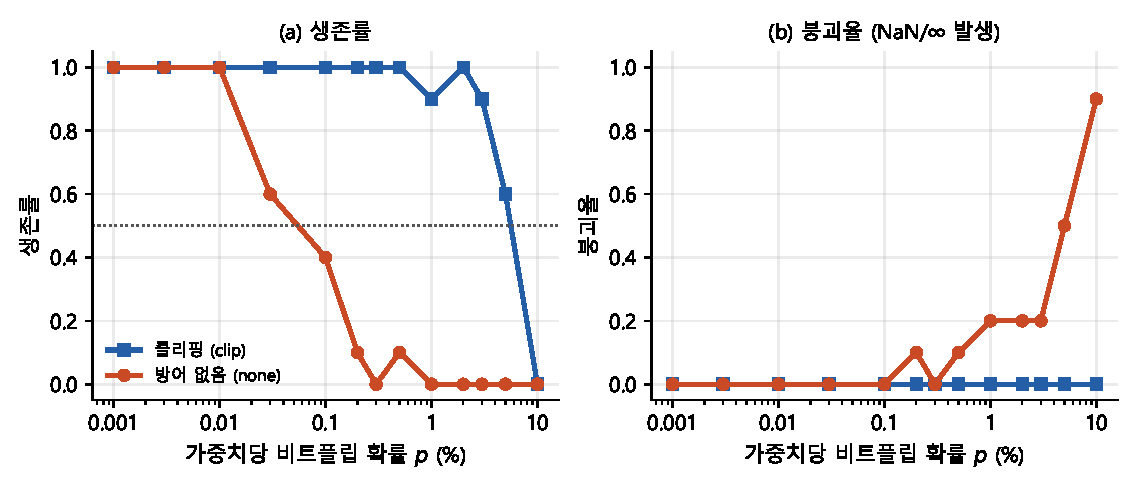
\includegraphics[width=0.95\linewidth]{fig_e1_survival_crash}
  \caption{(a) 생존률과 (b) 붕괴율. 점선은 생존률 50\,\%.}
  \label{fig:survival}
\end{figure}

\subsection{궤도에서의 날수로 바꾸면}
식~\eqref{eq:teq}로 바꾸면 \code{mnist\_linear}는 궤도에서 하루에 약 \LeoFlipsPerDay{}개의 가중치가 맞는다. 절반이 망가지는 시점은 방어 없음에서 약 \PhalfNoneDays{}일, 클리핑에서 약 \PhalfClipDays{}일이다. 아무 방어 없는 신경망은 몇 주 안에 절반의 확률로 성능이 10\,\% 넘게 떨어지지만, 가장 단순한 클리핑만 켜도 몇 년 단위가 된다.

\subsection{큰 모델이 먼저 망가진다: 생존을 정하는 것은 명중 수}
그림~\ref{fig:models}는 네 모델의 결과다. 가로축을 $p$로 두면 큰 모델일수록 곡선이 왼쪽에 있다. 같은 $p$에서 큰 모델이 먼저 망가진다는 뜻이다. 절반이 망가지는 $p$는 가장 작은 모델 \PhalfNoneLinear\,\%에서 가장 큰 모델 \PhalfNoneResnet\,\%로 약 50배 낮다. ``큰 모델이 더 튼튼하다''는 생각은 틀렸고, 예상 (마)가 맞았다.

그런데 가로축을 $p$ 대신 \textbf{명중 수} $k$로 바꾸면(그림~\ref{fig:models_hits}) 네 모델의 곡선이 거의 한 줄로 겹친다. 절반이 망가지는 명중 수 $k_{50}$은 \KhalfNoneLinear{}, \KhalfNoneCnn{}, \KhalfNoneCifar{}, \KhalfNoneResnet{}개다. 가중치 수가 110배 다른데 2배 안에 든다. 즉 생존을 정하는 것은 확률 $p$가 아니라 ``\emph{몇 개가 뒤집혔나}''이고, 그 수가 60--110개쯤 되면 bit~30 명중이 하나쯤 섞이기 때문에 어느 모델이든 무너진다.

\begin{figure}[!htb]
  \centering
  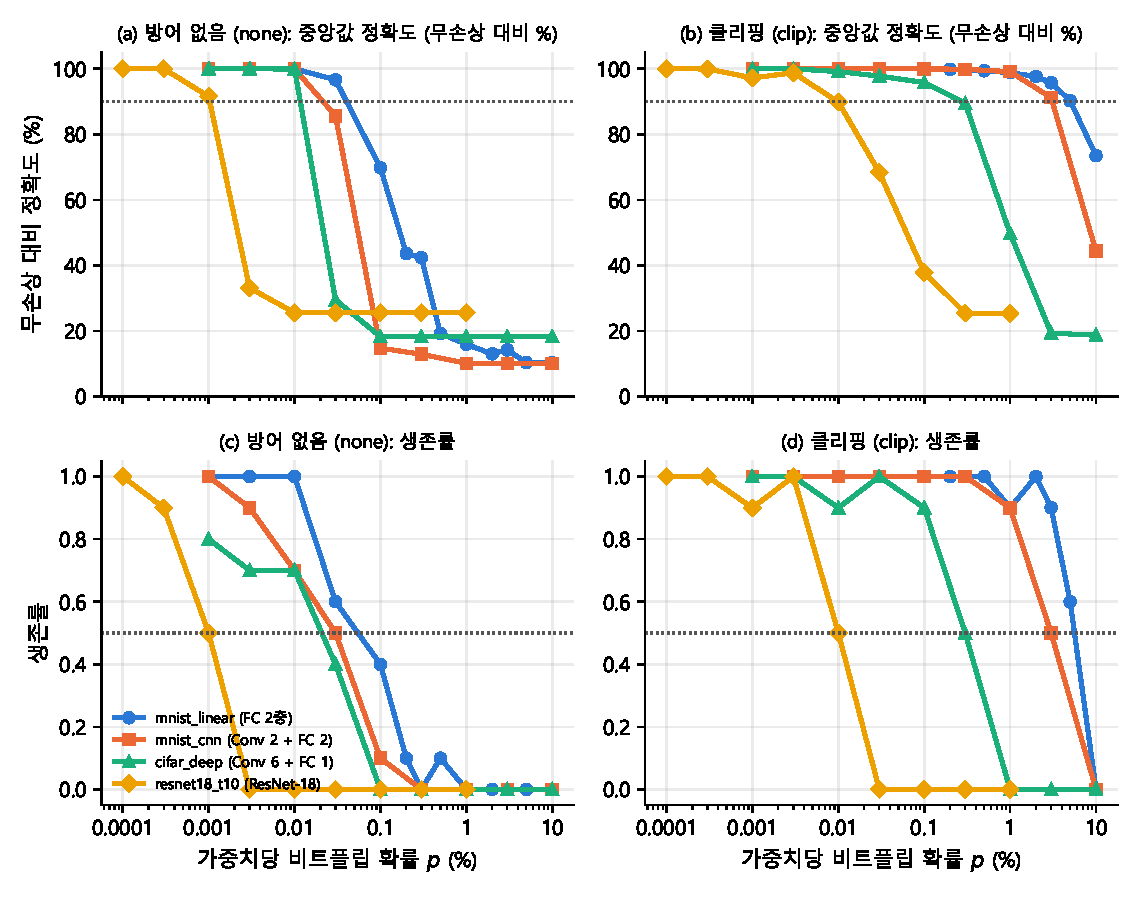
\includegraphics[width=0.95\linewidth]{fig_e1_models}
  \caption{E1-M: 네 모델의 $p$에 따른 결과. (a)(b) 깨끗할 때 대비 정답률 중앙값, (c)(d) 생존률. 왼쪽 열은 방어 없음, 오른쪽 열은 클리핑.}
  \label{fig:models}
\end{figure}

\begin{figure}[!htb]
  \centering
  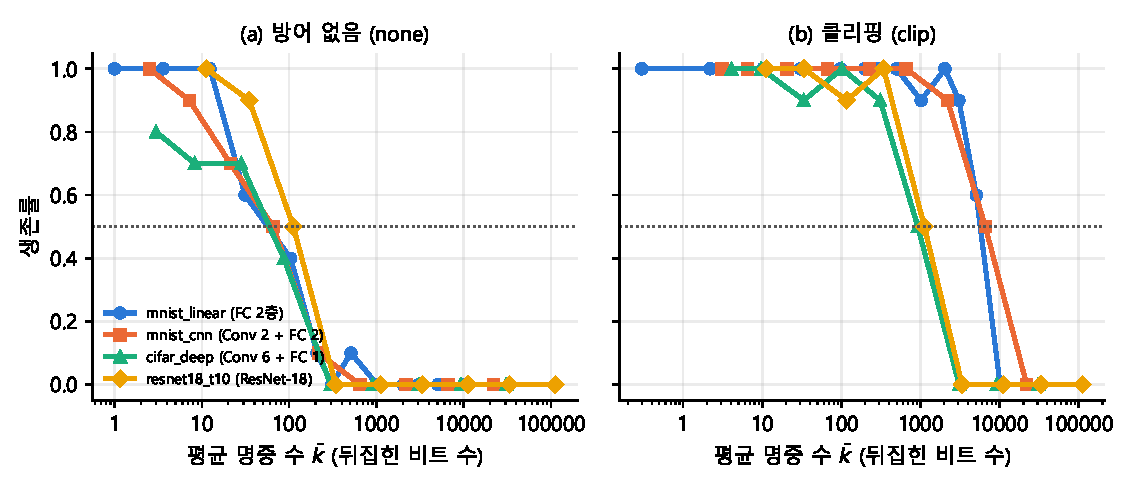
\includegraphics[width=0.95\linewidth]{fig_e1_models_hits}
  \caption{가로축을 명중 수로 바꾼 생존률. 방어 없음(a)에서는 네 모델이 한 곡선으로 모인다.}
  \label{fig:models_hits}
\end{figure}

이것이 궤도에서 뜻하는 바는 무겁다. 하루 명중 수는 비트 수에 비례하므로 큰 모델은 그만큼 자주 맞는다. 표~\ref{tab:model}에서 방어 없음의 날수는 \code{mnist\_linear} \DaysNoneLinear{}에서 \code{resnet18\_t10} \DaysNoneResnet{}으로 줄어든다. $k_{50}\approx60$--$110$을 그대로 적용하면 ResNet-50(2,560만 개)은 약 \TfiftyResnetFifty{}, 1억 개짜리 모델은 약 \TfiftyHundredMMin{}이다. 방어 없는 큰 신경망은 궤도에서 하루를 버티지 못한다.

클리핑의 이득은 모델마다 달랐다. MNIST 두 모델에서는 약 \ClipGainLinear{}배와 \ClipGainCnn{}배였지만, 깨끗할 때 정답률이 낮은 CIFAR-10 두 모델에서는 \ClipGainCifar{}배와 \ClipGainResnet{}배에 그쳤다. 클리핑은 무한대 붕괴는 완전히 막지만, $\pm3$으로 잘린 가중치 수백 개가 남기는 작은 손상은 막지 못한다. 원래 여유가 적은 모델은 그 작은 손상에도 더 예민하다.

\subsection{32칸 중 딱 한 칸만 위험하다}
E2에서는 정확히 한 칸만 한 번 뒤집었다. 결과(그림~\ref{fig:e2})는 아주 단순하다. \textbf{bit~30을 뺀 모든 칸에서 생존률은 1.00이었다.} 부호 칸은 가중치 하나의 부호만 바꾸고, 지수의 나머지 칸들은 학습된 가중치(대부분 $|w|<1$)에서 이미 1인 경우가 많아 뒤집히면 오히려 값이 작아지거나, 커져도 2--16배에 그쳐 수만 개의 합에 묻힌다. bit~30 한 번 명중의 생존률은 네 모델에서 \SthirtyEtwoLinear{}, \SthirtyEtwoCnn{}, \SthirtyEtwoCifar{}, \SthirtyEtwoResnet{}이었다. 단 한 번 맞았을 뿐인데 10번 중 2--5번은 망가진다는 뜻이다. 클리핑을 켜면 bit~30을 포함한 모든 칸에서 1.00이었다. 하나가 $\pm3$으로 잘리는 것은 아무 해가 없기 때문이다.

\begin{figure}[!htb]
  \centering
  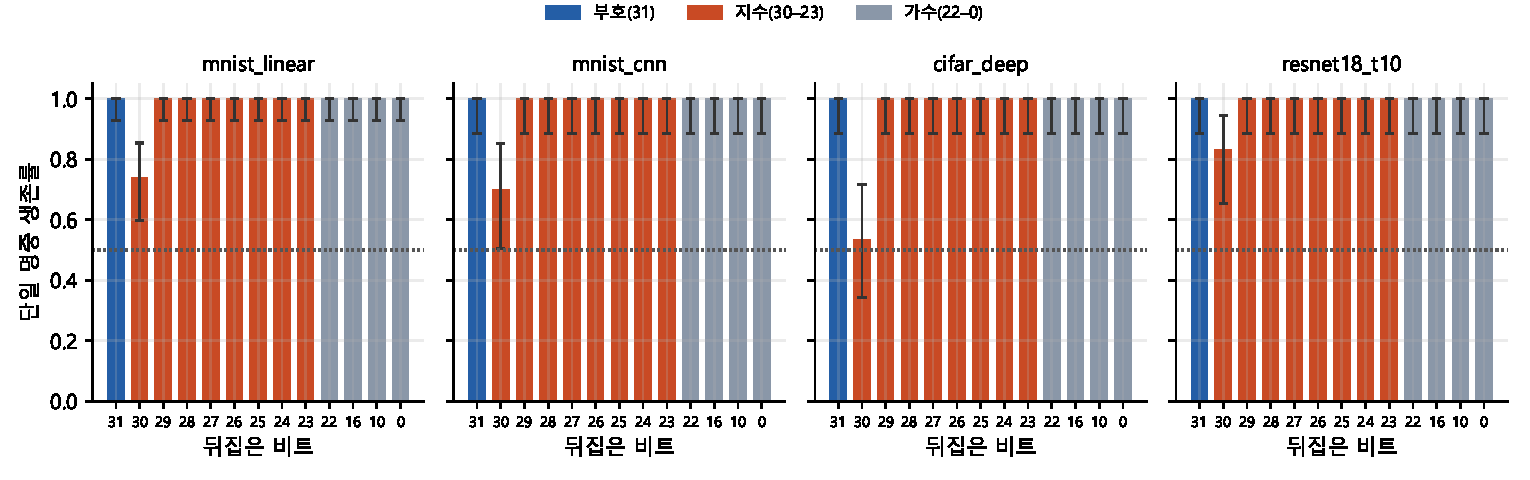
\includegraphics[width=0.95\linewidth]{fig_e2_bits}
  \caption{E2 비트 지도: 칸 하나를 딱 한 번 뒤집었을 때의 생존률(방어 없음). 막대는 95\,\% 신뢰구간. 32칸 가운데 bit~30만 위험하다.}
  \label{fig:e2}
\end{figure}

\subsection{방어 여섯 가지 비교}
그림~\ref{fig:e5}와 표~\ref{tab:e5}는 \code{mnist\_linear}에서 방어 6종을 비교한 것이다.
\begin{itemize}[leftmargin=*]
  \item \textbf{패리티와 TMR}은 $p=3\,\%$(명중 약 3,000개)까지 생존률 1.0이었다. $p$를 50\,\%까지 올려 보니(표~\ref{tab:e5high}) TMR은 $10\,\%$에서 0.8, $20\,\%$에서 0으로 무너졌다. 패리티는 가중치의 20\,\%가 0이 되어도 생존률 1.0(중앙값 92.3\,\%)이었고 30\,\%에서야 0.8이 되었다. 가장 강하면서 가장 싼(메모리 +3\,\%) 방어였다.
  \item \textbf{클리핑}의 이득은 약 \GainEClip{}배였다(E1의 \PhalfRatio{}배와 같은 자릿수).
  \item \textbf{앙상블(중앙값)}은 $p=0.1\,\%$까지 버티다 $0.3\,\%$에서 0으로 떨어져 이득이 \GainEEnsMed{}배에 그쳤다.
  \item \textbf{앙상블(평균)}은 이득 \GainEEns{}배로 \emph{방어 없음보다 나빴다}. 다섯 벌 중 하나라도 $10^{38}$을 내면 평균이 거기 끌려가는데, 벌이 다섯이니 그런 벌이 생길 확률도 다섯 배다. 그래서 혼자일 때의 $1/5$ 양에서 망가진다. 측정값 0.2배가 정확히 $1/5$이다.
\end{itemize}

\begin{figure}[!htb]
  \centering
  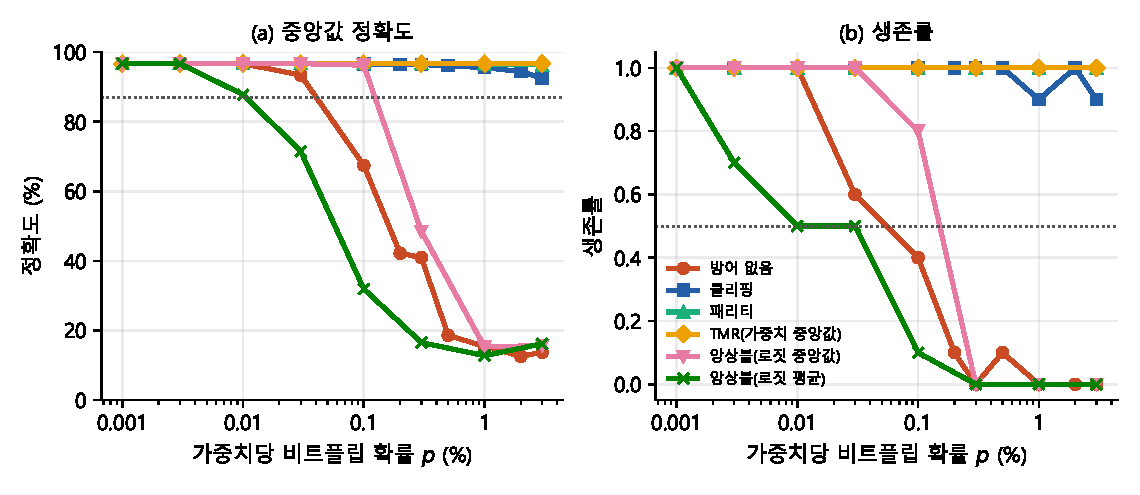
\includegraphics[width=0.95\linewidth]{fig_e5_defenses}
  \caption{E5: 방어 6종. (a) 정답률 중앙값, (b) 생존률. 패리티와 TMR은 겹쳐서 TMR 아래에 있다.}
  \label{fig:e5}
\end{figure}

\begin{table}[!htb]
  \centering\scriptsize
  \caption{E5 방어별 정답률 중앙값(괄호는 생존률)과 절반이 망가지는 명중 수 $k_{50}$, 이득(방어 없음의 $k_{50}$ 대비 몇 배인가).}
  \label{tab:e5}
  \setlength{\tabcolsep}{3pt}
\begin{tabular}{lrrrrrrrr|rr}
\toprule
방어 & $p$=0.001\% & $p$=0.003\% & $p$=0.01\% & $p$=0.03\% & $p$=0.1\% & $p$=0.3\% & $p$=1\% & $p$=3\% & $k_{50}$ & 이득 \\
\midrule
없음 & 96.7 (1.0) & 96.7 (1.0) & 96.6 (1.0) & 93.4 (0.6) & 67.4 (0.4) & 40.9 (0.0) & 15.4 (0.0) & 13.7 (0.0) & 62 & 1.0 \\
클리핑 & 96.7 (1.0) & 96.7 (1.0) & 96.7 (1.0) & 96.6 (1.0) & 96.6 (1.0) & 96.4 (1.0) & 95.5 (0.9) & 92.5 (0.9) & 5,155 & 83.8 \\
패리티 & 96.7 (1.0) & 96.7 (1.0) & 96.7 (1.0) & 96.7 (1.0) & 96.7 (1.0) & 96.6 (1.0) & 96.6 (1.0) & 96.3 (1.0) & 31,371 & 509.7 \\
TMR & 96.7 (1.0) & 96.7 (1.0) & 96.7 (1.0) & 96.7 (1.0) & 96.7 (1.0) & 96.7 (1.0) & 96.7 (1.0) & 96.7 (1.0) & 10,639 & 172.8 \\
앙상블(중앙값) & 96.7 (1.0) & 96.7 (1.0) & 96.7 (1.0) & 96.7 (1.0) & 96.2 (0.8) & 48.5 (0.0) & 15.3 (0.0) & 15.7 (0.0) & 109 & 1.8 \\
앙상블(평균) & 96.7 (1.0) & 96.7 (0.7) & 87.8 (0.5) & 71.5 (0.5) & 31.9 (0.1) & 16.5 (0.0) & 12.8 (0.0) & 16.2 (0.0) & 13 & 0.2 \\
\bottomrule
\end{tabular}

\end{table}

\begin{table}[!htb]
  \centering\scriptsize
  \caption{아주 많이 맞혔을 때의 TMR과 패리티(각 10번). ``TMR 예측''은 \ref{sec:model}절의 식으로 계산한 값.}
  \label{tab:e5high}
  \begin{tabular}{lrr|rr|rr}
\toprule
$p$ (\%) & $\bar{k}$ & $k/N_w$ & TMR 실측 & TMR 예측 & 패리티 실측 & 패리티 중앙값 \\
\midrule
0.001 & 1 & 0.00 & 1.0 & 1.00 & 1.0 & 96.7 \\
0.003 & 3 & 0.00 & 1.0 & 1.00 & 1.0 & 96.7 \\
0.01 & 10 & 0.00 & 1.0 & 1.00 & 1.0 & 96.7 \\
0.03 & 30 & 0.00 & 1.0 & 1.00 & 1.0 & 96.7 \\
0.1 & 102 & 0.00 & 1.0 & 1.00 & 1.0 & 96.7 \\
0.3 & 306 & 0.00 & 1.0 & 1.00 & 1.0 & 96.6 \\
1 & 1,021 & 0.01 & 1.0 & 0.99 & 1.0 & 96.6 \\
3 & 3,061 & 0.03 & 1.0 & 0.93 & 1.0 & 96.3 \\
5 & 5,108 & 0.05 & 1.0 & 0.81 & 1.0 & 96.1 \\
10 & 10,188 & 0.10 & 0.8 & 0.44 & 1.0 & 95.3 \\
20 & 20,331 & 0.20 & 0.0 & 0.04 & 1.0 & 92.3 \\
30 & 30,501 & 0.30 & 0.0 & 0.00 & 0.8 & 88.3 \\
50 & 50,842 & 0.50 & 0.0 & 0.00 & 0.0 & 74.2 \\
\bottomrule
\end{tabular}

\end{table}

\subsection{진짜 궤도처럼 몰려서 맞아도 같다}
E3에서는 하루 명중의 90\,\%를 SAA 통과 3번(각 12분)에 몰아넣었다. 결과는 같은 명중 수의 E1과 같았다(그림~\ref{fig:e3}). 방어 없는 \code{mnist\_linear}는 7일까지 생존률 0.9--1.0을 지키다가 30일에 0.3, 90일에 0.1로 떨어졌고, 클리핑은 90일까지 1.0이었다. 명중이 한꺼번에 들어오든 고르게 들어오든 결과가 같은 이유는, 우리 실험의 신경망이 ``다 맞은 뒤에'' 문제를 푸는 것이라 맞은 \emph{순서}가 상관없기 때문이다.

\begin{figure}[!htb]
  \centering
  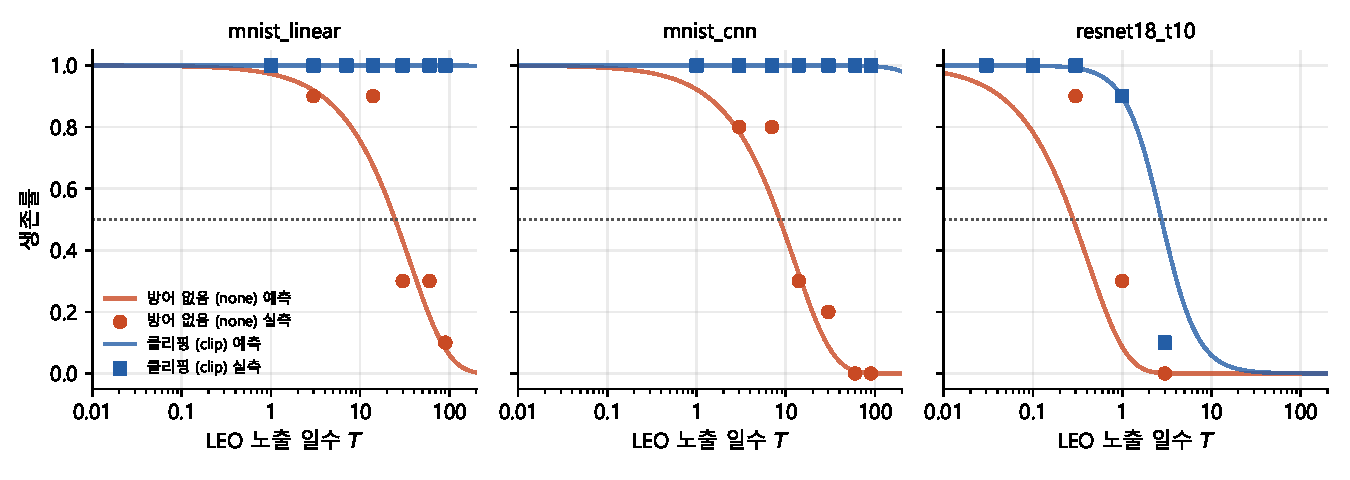
\includegraphics[width=0.95\linewidth]{fig_e3_leo}
  \caption{E3: 궤도 모드 실측 생존률(점)과 E1만 보고 세운 식의 예측(선). 식은 E3 데이터를 본 적이 없다.}
  \label{fig:e3}
\end{figure}

% ------------------------------------------------------------
\section{식 하나로 정리하기}
\label{sec:model}

\subsection{``한 번 맞아 망가질 확률'' $q$}
지금까지의 결과를 식 하나로 모아 보자. 명중 하나가 모델을 망가뜨릴 확률을 $q$라고 하자(``치명 확률''). 명중이 서로 독립이라면, $k$번 맞고도 살아남을 확률은 $k$번 모두 치명적이지 않을 확률이므로
\begin{equation}
  S(k)=(1-q)^{k}
  \label{eq:modelA}
\end{equation}
이다. 이것이 \textbf{모델 A}다.

\begin{easy}[주사위 게임]
주사위를 던져 1이 나오면 탈락하는 게임이다. 한 번 던져 살아남을 확률은 $5/6$, $k$번 던져 계속 살아남을 확률은 $(5/6)^k$다. 식~\eqref{eq:modelA}는 ``1이 나올 확률''을 $q$로 바꾼 것뿐이다. 모델에 따라 주사위의 면 수가 다를 뿐 게임은 같다.
\end{easy}

$q$는 세 가지가 모두 맞아떨어져야 하는 확률이라 세 수의 곱으로 쓸 수 있다.
\begin{equation}
  q=\frac{1}{32}\times\pi_+\times\alpha .
  \label{eq:q}
\end{equation}
\begin{itemize}[leftmargin=*,nosep]
  \item $1/32$: 명중이 하필 bit~30에 떨어질 확률. float32의 구조에서 정해진다.
  \item $\pi_+$(파이 플러스): 양수 가중치의 비율. $+10^{38}$은 다음 층을 지배하지만 $-10^{38}$은 ReLU라는 함수가 0으로 잘라 버려 대개 무해하다. 학습된 가중치에서 양수를 세어 보면 네 모델에서 0.42--0.49다.
  \item $\alpha$(알파): 그 가중치가 실제로 출력까지 이어지는 길 위에 있을 비율. 예컨대 손글씨 사진의 테두리처럼 늘 0인 픽셀에 붙은 가중치는 아무리 커져도 출력에 닿지 않는다. 이 값은 일일이 셀 수 없어 E1 데이터에 식을 맞춰 구했다. 네 모델에서 \AlphaMin{}--\AlphaMax{}다.
\end{itemize}

\begin{calc}[\code{mnist\_linear}의 $q$와 ``절반이 망가지는 명중 수'']
\code{mnist\_linear}는 $\pi_+=0.49$, $\alpha=\AlphaLinear$이므로 $q=\frac{1}{32}\times0.49\times\AlphaLinear\approx\QLinear$이다. 약 120번에 한 번꼴로 치명적이라는 뜻이다. 절반이 망가지는 명중 수는 $(1-q)^k=1/2$를 푸는 것인데, $q$가 작을 때 답은 약 $0.69/q$이다(0.69는 $\ln2$라는 상수). $0.69/\QLinear\approx80$이다. 실제로 잰 $k_{50}$은 \KhalfNoneLinear{}개였다. 네 모델의 $q$는 \QMin{}--\QMax{}로 2.4배 안에 들어, ``치명 확률은 모델 크기와 거의 무관하다''는 예상 (라)와 맞는다.
\end{calc}

\subsection{식이 맞는지 세 가지로 확인했다}
\begin{enumerate}[leftmargin=*]
  \item \textbf{한 칸 실험(E2)과 맞는가.} bit~30 한 번 명중의 생존률은 식으로는 $1-\pi_+\alpha=1-32q$이다. E1으로 구한 $q$를 넣으면 네 모델에서 \SthirtyPredLinear{}, \SthirtyPredCnn{}, \SthirtyPredCifar{}, \SthirtyPredResnet{}이고, E2에서 실제로 잰 값은 \SthirtyEtwoLinear{}, \SthirtyEtwoCnn{}, \SthirtyEtwoCifar{}, \SthirtyEtwoResnet{}이다. 모두 신뢰구간 안에 들었다. 수십 개가 무작위로 맞을 때의 붕괴와 딱 한 칸의 위험이 같은 수 $q$로 이어진다.
  \item \textbf{궤도 모드(E3)를 예측하는가.} E1 데이터로만 맞춘 식으로 E3의 생존률을 예측했더니 \EthreeN{}개 조건에서 평균 오차 \EthreeMAE{}였다(그림~\ref{fig:e3}의 선).
  \item \textbf{TMR의 한계를 예측하는가.} TMR에서 가중치 하나가 망가지려면 세 벌 중 두 벌이 \emph{같은} 가중치의 bit~30을 맞아야 한다. 그래서 치명 수가 $k$가 아니라 $k^2$에 비례하고, 절반이 망가지는 명중 수는 $\sqrt{32N_w\ln2/(3q)}$가 된다. \code{mnist\_linear}에 넣으면 약 \KfiftyTmrPred{}개($p\approx\PfiftyTmrPred\,\%$)이고, 실험에서 TMR은 $p=10\,\%$에서 0.8, $20\,\%$에서 0으로 무너졌다(표~\ref{tab:e5high}). 같은 논리로 평균 앙상블은 다섯 벌 중 하나라도 치명이면 끝이므로 이득이 $1/5$로 예측되고, 실측은 \GainEEns{}배였다.
\end{enumerate}

\subsection{식으로 무엇을 할 수 있나}
이제 어떤 모델이든 궤도에서 버티는 시간을 계산할 수 있다. 하루 명중 수는 $r\times32\times N_w$이므로 절반이 망가지는 시간은 $T_{50}\approx0.69/(q\times r\times32N_w)$이다. $q\approx0.01$을 쓰면 ResNet-50은 약 \TfiftyResnetFifty{}, 1억 개짜리 모델은 약 \TfiftyHundredMMin{}이다. 클리핑을 켜면 여유가 큰 과제에서 약 100배, 여유가 작은 과제에서 10--15배 늘어난다. 거꾸로 ``임무 기간 $T$ 동안 생존률 $S^\ast$ 이상''이라는 조건을 주면, 그 조건을 만족하는 최대 모델 크기를 바로 구할 수 있다.

% ------------------------------------------------------------
\section{이 연구의 한계}
\begin{itemize}[leftmargin=*]
  \item \textbf{가중치만 뒤집었다.} 계산 중간값, 학습 중의 기울기, 프로그램 코드가 든 메모리의 비트플립은 다루지 않았다. 한 번에 여러 칸이 뒤집히는 경우도 빼놓았다.
  \item \textbf{$r$은 두 위성의 측정값으로 고정했다.} 실제 SEU 발생률은 메모리 종류, 고도, 차폐, 태양 활동에 따라 수십 배에서 수천 배까지 달라진다. 날수는 ``$r=10^{-6}$일 때''의 값으로 읽어야 한다.
  \item \textbf{float32만 실험했다.} 실제 위성용 신경망은 정수형(int8)을 많이 쓰는데, 정수형에는 지수 칸이 없어 결과가 다를 수 있다.
  \item \textbf{큰 두 모델은 깨끗할 때 정답률이 낮다.} 컴퓨터 시간이 모자라 \code{cifar\_deep}과 \code{resnet18\_t10}은 \CleanCifar{}\,\%, \CleanResnet{}\,\%에 그쳤다. ``여유가 적은 모델''의 결과로 읽어야 하며, 충분히 학습하면 클리핑의 이득이 더 클 수 있다.
  \item \textbf{반복이 10번이다.} 10번 중 6번 살아남았을 때 참 생존률은 대략 0.3--0.85 사이 어디든 될 수 있다. 그래서 이봉 분포 그림만은 100번씩 반복했다.
  \item \textbf{$\alpha$는 데이터에 맞춘 값이다.} $1/32$와 $\pi_+$는 직접 셌지만 $\alpha$는 그렇지 않다. 다만 E2에서 독립적으로 잰 값과 맞는 것으로 확인했다.
\end{itemize}

% ------------------------------------------------------------
\section{결론과 다음 연구}
우주 방사선이 인공신경망의 숫자 한 칸을 바꾸면 무슨 일이 생기는가? 답은 ``어느 칸이냐에 달렸다''이다. 32칸 중 31칸은 바뀌어도 거의 아무 일이 없고, 지수 맨 윗칸 하나만 숫자를 $10^{38}$배로 만들어 모델을 통째로 망가뜨린다. 그래서 정답률은 서서히 떨어지지 않고 어느 순간 갑자기 무너지며, 같은 양을 맞아도 운명이 둘로 갈린다. 생존을 정하는 것은 확률이 아니라 \emph{몇 개가 뒤집혔나}이고, 그 한계치는 모델 크기와 상관없이 60--110개쯤이다. 따라서 자리가 많아 더 자주 맞는 큰 모델이 먼저 망가지고, ResNet-18급 모델은 방어 없이 궤도에서 하루를 못 버틴다. 이 모든 것이 ``한 번 맞아 망가질 확률 $q\approx1/100$''과 식 $S=(1-q)^k$로 정리되며, 식은 보지 않은 궤도 실험도 맞혔다.

실용적인 결론은 분명하다. 위성에 신경망을 실을 때는 \textbf{최소한 클리핑을 켜야 한다}. 비용이 거의 없는데 버티는 시간을 MNIST 모델에서 약 100배, 여유가 적은 모델에서도 10배 넘게 늘려 준다. 더 튼튼하게 만들려면 패리티나 TMR을 쓰되, 모든 칸이 아니라 위험한 bit~30만 골라 보호하면 비용을 크게 줄일 수 있을 것이다. 이것을 확인하는 것이 다음 연구다.

다음에 하고 싶은 일은 이렇다.
\begin{enumerate}[leftmargin=*,nosep]
  \item bit~30만 골라서 패리티·TMR로 보호하는 ``선택 보호''의 이득과 비용을 재기.
  \item 학습이 끝난 뒤가 아니라 \emph{학습 중에} 비트가 뒤집히면 어떻게 되는지 보기.
  \item 정수형(int8) 모델과, 충분히 학습된 CIFAR-10 모델에서 같은 실험을 반복하기.
\end{enumerate}

% ------------------------------------------------------------
\section*{직접 해 보기}
모든 코드와 결과 파일은 \url{https://github.com/SJinLee/AI-in-space}에 있다. 보통 노트북(CPU)으로 몇 분이면 E1을 다시 돌릴 수 있다.
\begin{quote}\small
\code{python src/simulate.py --model mnist\_linear --mode infer --rad stress \textbackslash}\\
\code{\hspace*{2em}--p 0.001 --defense none --trials 10}
\end{quote}
이 글과 원 논문의 그림·표·숫자는 모두 \code{python paper/make\_figures.py}가 결과 파일에서 자동으로 다시 만든다.

\bibliographystyle{IEEEtranN}
\bibliography{refs}

% ------------------------------------------------------------
\appendix
\section{용어 사전}
\begin{table}[H]
  \centering\small
  \begin{tabular}{lp{11.2cm}}
    \toprule
    낱말 & 뜻 \\
    \midrule
    비트(bit) & 0 아니면 1을 저장하는 메모리의 가장 작은 칸. \\
    비트플립 & 비트 하나가 0에서 1로, 또는 1에서 0으로 뒤집히는 것. \\
    SEU & 단일 사건 오류. 방사선 입자 하나가 비트 하나를 뒤집는 일. 고장이 아니라 값만 바뀐 것. \\
    저궤도(LEO) & 고도 수백\,km의 지구 궤도. 국제우주정거장과 대부분의 관측 위성이 여기 있다. \\
    SAA & 남대서양 이상 지역. 지구 자기장이 약해 방사선이 많이 내려오는 곳. 저궤도 위성이 하루 몇 번 지난다. \\
    float32 & 소수를 32칸(부호 1, 지수 8, 가수 23)으로 저장하는 방식. \\
    지수(E), 가수(M) & 과학적 표기법 $6.02\times10^{23}$에서 23이 지수, 6.02가 가수에 해당. \\
    bit 30 & float32의 지수 맨 윗칸. 이 칸이 뒤집히면 값이 $10^{38}$배 또는 무한대가 된다. \\
    NaN & ``숫자 아님''. $\infty-\infty$처럼 답을 정할 수 없는 계산의 결과. 섞이면 전염된다. \\
    인공신경망 & 곱하고 더하기를 층층이 쌓아 입력에서 답을 내는 프로그램. 가중치라는 숫자 수십만 개로 이루어진다. \\
    가중치(weight) & 신경망이 입력에 곱하는 숫자. 학습으로 정해지고 메모리에 저장된다. \\
    ReLU & 음수는 0으로, 양수는 그대로 두는 함수. 신경망의 층 사이에 들어간다. \\
    $p$ & 가중치 하나가 명중될 확률. 실험에서 방사선 양을 조절하는 손잡이. \\
    $r$ & 비트 하나가 하루에 뒤집힐 확률. 궤도에서 실제로 잰 값으로 약 $10^{-6}$. \\
    명중 수 $k$ & 한 번 실험에서 실제로 뒤집힌 가중치의 수. 평균 $k=p\times$가중치 수. \\
    정답률 & 시험 문제 1만 장 중 맞힌 비율(\%). \\
    생존 & 붕괴하지 않고 정답률이 깨끗할 때의 90\,\% 이상인 것. 생존률은 10번 중 살아남은 비율. \\
    붕괴 & 가중치나 출력에 NaN 또는 무한대가 생긴 것. \\
    중앙값 & 값을 크기 순으로 늘어놓았을 때 가운데 값. 평균과 달리 큰 값 하나에 끌려가지 않는다. \\
    이봉 분포 & 봉우리가 둘인 분포. 결과가 ``멀쩡''과 ``망가짐''의 두 무리로 갈릴 때 나온다. \\
    클리핑 & 너무 큰 값을 정해진 범위($\pm3$)로 잘라 내는 방어. \\
    패리티 & 1의 개수가 짝수가 되도록 한 칸을 더 붙여 오류를 알아내는 방법. \\
    TMR & 같은 값을 세 벌 저장하고 중앙값을 쓰는 방어. \\
    앙상블 & 모델 여러 벌의 답을 평균이나 중앙값으로 합치는 방법. \\
    $q$ & 명중 하나가 모델을 망가뜨릴 확률. 네 모델에서 약 $1/100$. \\
    $k_{50}$, $p_{50}$, $T_{50}$ & 생존률이 절반이 되는 명중 수, $p$, 궤도 날수. \\
    이득 & 방어를 켰을 때 버틸 수 있는 양이 몇 배가 되는가. \\
    \bottomrule
  \end{tabular}
\end{table}

\end{document}
